%%%%%%%%%%%%%%%%%%%%%%%%%%%%%%%%%%%%%%%%%%%%%%%%%%%%%%%%%%%%%%%%%%%%%%
\section{テスト定義}
\label{sec:test}

この節では, 最初の4節で4つのモジュール, すなわち通信用データクラス,領
域クラス, 粒子群クラス, 相互作用ツリークラスのテストについて記述する。
様々なデータ構造が現れるが, 断らないかぎり, そのデータ構造はそのクラス
に属す。最後に結合テストについて記す。


%%%%%%%%%%%%%%%%%%%%%%%%%%%%%%%%%%%%%%%%%%%%%%
\subsection{通信用データクラス}

%%%%%%%%%%%%%%%%%%%%%%%%%%%%%%%%%%%%%%%%%%%%%%
\subsection{領域クラス}

%%%%%%%%%%%%%%%%%%%%%%%%%%%%%%%%%%%%%%%%%%%%%%
\subsection{粒子群クラス}

\subsection{リアル粒子の交換}

交換前と交換後で粒子の個数が変わっていないかをチェック. 交換後に, プロ
セスが担当する粒子が適切かどうかチェック.


%%%%%%%%%%%%%%%%%%%%%%%%%%%%%%%%%%%%%%%%%%%%%%
\subsection{相互作用ツリークラス}

\subsubsection{ソートの単体テスト}

\begin{lstlisting}[caption=radix sortのテスト]
int main(int argc, char *argv[]){

    if(argc < 3){
        std::cerr<<"too few args.; arg1: problem size, arg2: repeat count"<<std::endl;
        return 1;
    }

    PS::RadixSort<PS::U64, 8> RS;

    PS::S32 n_size = std::atoi(argv[1]);
    PS::S32 n_repeat = std::atoi(argv[2]);
    PS::TreeParticle * data = new PS::TreeParticle[n_size];
    PS::TreeParticle * data_buf = new PS::TreeParticle[n_size];
    bool * flag = new bool[n_size];
    PS::S32 err_comp = 0;
    PS::S32 err_order = 0;

    for(PS::S32 i=0; i<n_repeat; i++){
        for(int j=0; j<n_size; j++){
            data[j].setKey(PS::U64(abs(rand()))<<32 | PS::U64(abs(rand())));
            data[j].adr_ptcl_ = j;
            flag[j] = false;
        }
        RS.lsdSort(data, data_buf, 0, n_size-1);
        for(PS::S32 j=0; j<n_size; j++) flag[data[j].adr_ptcl_] = true;
        for(PS::S32 j=0; j<n_size; j++){
            if(flag[j] == false){
                err_comp++;
            }
        }
        for(PS::S32 j=1; j<n_size; j++){
            if(data[j].getKey() < data[j-1].getKey() ){
                err_order++;
            }
        }
    }

    if( err_comp || err_order){
        std::cout<<"FAIL err_comp="<<err_comp<<" err_order="<<err_order<<std::endl;
    }
    else{
        std::cout<<"PASS"<<std::endl;
    }

    return 0;
}
\end{lstlisting}

コマンドラインから第一引数が問題サイズ、第二引数が繰り返し回数。ソート
された配列を先頭から見ていき、常に次の値が現在の値より大きいかをチェッ
クし、また粒子が消えたりしていないかもチェックする。


\subsubsection{ローカルツリーのモートンソート}

モートン順序に並べられた{\tt EPI}から再びモートンキーを作り、モートンオー
ダーにならんでいるかをチェックする。また、モートンオーダーに並べたとき
に粒子が消えたりしていないかを{\tt TP}の{\tt adr\_ptc\_}を見ることでチェッ
クする。このテストは以下の関数によって行われる。結果の出力は{\tt fout}
に行う。

\begin{screen}
\begin{verbatim}
void checkMortonSortLocalTreeOnly(std::ostream & fout = std::cout){
\end{verbatim}
\end{screen}

\subsubsection{ローカルツリーの構築}

ローカルツリー内の全てのセルについて、各セルの持つ粒子がそのセルの境界
に入っているかをチェックする。セルの辿り方はツリーウォークと同じ方法で
行う。このテストは以下の関数によって行われる。第一引数{\tt tolerance}は
粒子がボックスから外れていた時に許容する大きさ。これは、ツリーの構築時
に使ったセルの大きさの定義とこの関数内での定義が丸め誤差の範囲では違い、
セル境界付近の粒子がボックスから出ていることがある為。結果の出力は{\tt
fout}に行う。

\begin{screen}
\begin{verbatim}
void checkMakeLocalTree(const F32 tolerance = 1e-6, std::ostream & fout = std::cout);
\end{verbatim}
\end{screen}

\subsubsection{ローカルツリーのモーメント計算}

モーメント計算のテストは以下の関数によって行う。サーチの種類により、行
うテストは異なる。結果は{\tt fout}に出力される。{\tt tolerance}は許容す
る誤差である。

\begin{screen}
\begin{verbatim}
void checkCalcMomentLocalTree(const F32 tolerance = 1e-5, std::ostream & fout = std::cout);
\end{verbatim}
\end{screen}

\subsubsubsection{長距離力、カットオフなし}

各プロセスの持つ全粒子の質量、重心を直接求め、それをモーメント計算によっ
て求めたツリーのルートセルのもつ質量、重心と比較する。{\tt tolerance}は
重心の質量、座標の差の許容誤差である。

\subsubsubsection{長距離力、カットオフあり}

\subsubsubsection{短距離力}

各プロセスの持つ全粒子の外側境界、内側境界を直接求め、それをモーメント
計算によって求めたツリーのルートセルのもつ外側境界、内側境界と比較する。
{\tt tolerance}はそれぞれの方法で求めた境界の許容誤差である。

\subsubsection{LET交換}

LET交換のテストは以下の関数によって行う。サーチの種類により、行うテスト
は異なる。結果は{\tt fout}に出力される。{\tt tolerance}は許容する誤差で、
長距離力の場合のみ必要である(短距離力の場合は無視される)。


\begin{screen}
\begin{verbatim}
void checkExchangeLocalEssentialTree(const DomainInfo & dinfo, const F32 tolerance = 1e-5, std::ostream & fout = std::cout){
\end{verbatim}
\end{screen}

\subsubsubsection{長距離力、カットオフなし}

自プロセスの{\tt EPJ}と送られて来た{\tt EPJ}、{\tt SPJ}から、重心を計算
し、その結果を全粒子の重心と比較する。全粒子の重心は、各プロセスで重心
を計算し、{\tt Allreduce}により求める。{\tt tolerance}は重心の質量、座
標の差の許容誤差である。

\subsubsubsection{長距離力、カットオフあり}

\subsubsubsection{短距離力、全モード}

送られて来た{\tt EPJ}とツリーを使わずに通信した場合に送られてきた{\tt
EPJ}とを比較する。比較は粒子のx座標を使ってソートし、二つの方法で送られ
て来た粒子の座標を比較する。

\subsubsection{グローバルツリーのモートンソート}

ローカルツリーのモートンソートのテストと同様に、モートン順序に並べられ
た{\tt EPI}から再びモートンキーを作り、モートンオーダーにならんでいるか
をチェックする。また、モートンオーダーに並べたときに粒子が消えたりして
いないかを{\tt TP}の{\tt adr\_ptc\_}を見ることでチェックする。このテス
トは以下の関数によって行われる。結果の出力は{\tt fout}に行う。

\begin{screen}
\begin{verbatim}
void checkMortonSortGlobalTreeOnly(std::ostream & fout = std::cout){
\end{verbatim}
\end{screen}

\subsubsection{グローバルツリーの構築}

ローカルツリーのテストと同様に、グローバルツリー内の全てのセルについて、
各セルの持つ粒子がそのセルの境界に入っているかをチェックする。セルの辿
り方はツリーウォークと同じ方法である。これは以下の関数で行う。

\begin{screen}
\begin{verbatim}
void checkMakeLocalTree(const F32 tolerance = 1e-6, std::ostream & fout = std::cout);
\end{verbatim}
\end{screen}

\subsubsection{グローバルツリーのモーメント計算}

モーメント計算のテストは以下の関数によって行う。サーチの種類により、行
うテストは異なる。結果は{\tt fout}に出力される。{\tt tolerance}は許容す
る誤差である。

\begin{screen}
\begin{verbatim}
void checkCalcMomentGlobalTree(const F32 tolerance = 1e-5, std::ostream & fout = std::cout);
\end{verbatim}
\end{screen}

\subsubsubsection{長距離力、カットオフなし}

各プロセスの持つ全粒子の質量、重心を直接求め、Allreduceし全体の重心質量、
座標を求め、それをモーメント計算によって求めたツリーのルートセルのもつ
質量、重心と比較する。{\tt tolerance}は重心の質量、座標の差の許容誤差で
ある。

\subsubsubsection{長距離力、カットオフあり}

\subsubsubsection{短距離力}

各プロセスの持つ全粒子の外側境界、内側境界を直接求め、それをモーメント
計算によって求めたツリーのルートセルのもつ外側境界、内側境界と比較する。
{\tt tolerance}はそれぞれの方法で求めた境界の許容誤差である。

\subsubsection{相互作用計算}

{\tt FDPS}で実際に求めた力と全粒子から直接求めた力を比較する。

\begin{screen}
\begin{verbatim}
template<class Tfunc_ep_ep, class Tfunc_compare>
void checkForce(Tfunc_ep_ep pfunc_ep_ep, Tfunc_compare func_compare,
                std::ostream & fout=std::cout);
\end{verbatim}
\end{screen}

ここで、{\tt pfunc\_ep\_ep}は計算で使うEPI-EPJ相互作用の関数、{\tt
func\_compare}は比較用の関数で、ユーザーが関数ポインタもしくはファンクタ
によって与えることが出来る。結果は{\tt fout}に出力する。\redtext{構造体
を返せた方が良い?}

{\tt func\_compare}は以下の様に定義出来る。
\begin{lstlisting}[caption=力の比較用ファンクタ]
struct CompareGrav{
    void operator () (ForceGrav * grav0, ForceGrav * grav1, 
                      const PS::S32 n, std::ostream & fout){
        bool err = false;
        for(PS::S32 i=0; i<n; i++){
            PS::F64 dpot = std::abs( (grav0[i].pot - grav1[i].pot) / grav0[i].pot );
            PS::F64vec dacc_vec = grav0[i].acc - grav1[i].acc;
            PS::F64 dacc = sqrt( (dacc_vec*dacc_vec) / (grav0[i].acc*grav0[i].acc) );
            if( dpot > 1e-1 || dacc > 1e-1){
                fout<<"Compare Grav: FAIL"<<std::endl;
                fout<<"grav0[i].pot="<<grav0[i].pot<<" grav1[i].pot="<<grav1[i].pot<<std::endl;
                fout<<"grav0[i].acc="<<grav0[i].acc<<" grav1[i].acc="<<grav1[i].acc<<std::endl;
                err = true;
            }
        }
        if(!err) fout<<"Compare Grav: PASS"<<std::endl;
    }
};
\end{lstlisting}[caption=]

また、ユーザーは以下の関数によって直接計算した力の値を得ることが出来る。
\begin{screen}
\begin{verbatim}
template<class Tfunc_ep_ep>
void calcForceDirect(Tfunc_ep_ep pfunc_ep_ep, Tforce force[], const bool clear=true);
\end{verbatim}
\end{screen}
{\tt force}は直接計算した力を格納する配列でユーザーが配列を確保する。
{\tt clear}は{\tt force}の値を初期化するかを決める。

これとFDPSで計算した力を返す関数を使う事で比較を行う事も出来る。
\begin{screen}
\begin{verbatim}
Tforce getForce(const S32 i);
\end{verbatim}
\end{screen}

以下に開放境界の場合の各関数のテストを記述する。

\begin{lstlisting}[caption=開放境界、モートンソート、ローカルツリー構築、モーメント計算、LET交換、グローバルツリー構築、相互作用計算のテスト]
int main(int argc, char *argv[]){
    std::cout<<std::setprecision(15);
    std::cerr<<std::setprecision(15);
    PS::Initialize(argc, argv);

    char sinput[1024];
    int c;
    while((c=getopt(argc,argv,"i:h")) != -1){
        switch(c){
        case 'i':
            sprintf(sinput,optarg);
            break;
        case 'h':
            std::cerr<<"i: input file name (nemo ascii)"<<std::endl;
            return 0;
        }
    }

    PS::ParticleSystem<FPGrav> system_grav;
    system_grav.initialize();
    PS::S32 n_grav_glb, n_grav_loc;
    PS::F32 time_sys;
    ReadNemoAscii(system_grav, n_grav_glb, n_grav_loc, time_sys, sinput);

    PS::DomainInfo dinfo;
    dinfo.initialize();
    dinfo.setBoundaryCondition(PS::BOUNDARY_CONDITION_OPEN);
    dinfo.collectSampleParticle(system_grav);
    dinfo.decomposeDomain();

    system_grav.exchangeParticle(dinfo);
    n_grav_loc = system_grav.getNumberOfParticleLocal();

#if 1
    PS::TreeForForceLong<ForceGrav, EPIGrav, EPJGrav, MomentGrav, SPJ>::Normal tree_grav;

    PS::F32 theta = 0.4;
    tree_grav.initialize(n_grav_glb, theta);
#if 0

#else
    //tree_grav.initializeLocalTree(half_len_grav_glb);
    tree_grav.setParticleLocalTree(system_grav);

    //tree_grav.mortonSortLocalTreeOnly(dinfo);
    tree_grav.setRootCell(dinfo);
    tree_grav.mortonSortLocalTreeOnly();
    tree_grav.checkMortonSortLocalTreeOnly();

    tree_grav.linkCellLocalTreeOnly();
    tree_grav.checkMakeLocalTree();

    tree_grav.calcMomentLocalTreeOnly();
    tree_grav.checkCalcMomentLocalTree();

    tree_grav.exchangeLocalEssentialTree(dinfo);
    tree_grav.checkExchangeLocalEssentialTree(dinfo);

    tree_grav.setLocalEssentialTreeToGlobalTree();

    tree_grav.mortonSortGlobalTreeOnly();
    tree_grav.checkMortonSortGlobalTreeOnly();

    tree_grav.linkCellGlobalTreeOnly();
    tree_grav.checkMakeGlobalTree();

    tree_grav.calcMomentGlobalTreeOnly();
    tree_grav.checkCalcMomentGlobalTree();

    tree_grav.makeIPGroup();
    tree_grav.checkMakeIPGroup();

    PS::S32 n_ipg_grav = tree_grav.getNumberOfIPG();
    bool err_grav = false;
    for(PS::S32 i=0; i<n_ipg_grav; i++){
        tree_grav.makeInteractionList(i, err_grav);
        //tree_grav.checkMakeInteractionList();
        tree_grav.calcForceOnly(CalcForceEpEp(), CalcForceSpEp(), i);
    }
    tree_grav.copyForceOriginalOrder();
    tree_grav.checkForce( CalcForceEpEp(), CompareGrav(), dinfo);

#endif
#endif


    ///////////////
    //// SHORT ////
    PS::ParticleSystem<FPSPH> system_sph;
    system_sph.initialize();
    PS::S32 n_sph_glb, n_sph_loc;
    ReadNemoAscii(system_sph, n_sph_glb, n_sph_loc, time_sys, sinput);
    PS::F64 half_len_sph_glb = system_sph.getHalfLength();
    std::cout<<"half_len_sph_glb="<<half_len_sph_glb<<std::endl;

    for(PS::S32 i=0; i<n_sph_loc; i++){
        system_sph[i].r_search = pow( (n_sph_glb/(half_len_sph_glb*half_len_sph_glb*half_len_sph_glb)), -0.333333) * (system_sph[i].id%10)*0.2;
    }

    system_sph.exchangeParticle(dinfo);
    n_sph_loc = system_sph.getNumberOfParticleLocal();

#if 0
    //////////////////////
    //// SCATTER MODE ////
    PS::TreeForForceShort<ResultDens, EPIScatter, EPJScatter>::Scatter tree_scatter;
    tree_scatter.initialize(n_sph_glb);
#if 0
    tree_scatter.calcForceAllAndWriteBack(CalcDensityScatter(), system_sph, dinfo);
    tree_scatter.checkForce( CalcDensityScatter(), CompareDensity(), dinfo);
#else

    tree_scatter.setParticleLocalTree(system_sph);

    tree_scatter.setRootCell(dinfo);
    tree_scatter.mortonSortLocalTreeOnly();
    tree_scatter.checkMortonSortLocalTreeOnly();

    tree_scatter.linkCellLocalTreeOnly();
    tree_scatter.checkMakeLocalTree();

    tree_scatter.calcMomentLocalTreeOnly();
    tree_scatter.checkCalcMomentLocalTree();

    tree_scatter.exchangeLocalEssentialTree(dinfo);
    tree_scatter.checkExchangeLocalEssentialTree(dinfo);

    tree_scatter.setLocalEssentialTreeToGlobalTree();

    tree_scatter.mortonSortGlobalTreeOnly();
    tree_scatter.checkMortonSortGlobalTreeOnly();

    tree_scatter.linkCellGlobalTreeOnly();
    tree_scatter.checkMakeGlobalTree();

    tree_scatter.calcMomentGlobalTreeOnly();
    tree_scatter.checkCalcMomentGlobalTree();

    tree_scatter.makeIPGroup();
    tree_scatter.checkMakeIPGroup();
    

    PS::S32 n_ipg_sph = tree_scatter.getNumberOfIPG();
    bool err_sph = false;
    for(PS::S32 i=0; i<n_ipg_sph; i++){
        tree_scatter.makeInteractionList(i, err_sph);
        tree_scatter.calcForceOnly( CalcDensityScatter(), i);
    }
    tree_scatter.copyForceOriginalOrder();

    tree_scatter.checkForce( CalcDensityScatter(), CompareDensity(), dinfo);

#endif
#endif

#if 0
    /////////////////////
    //// GATHER MODE ////
    PS::TreeForForceShort<ResultDens, EPIGather, EPJGather>::Gather tree_gather; 
    tree_gather.initialize(n_sph_glb);
#if 0
    tree_gather.calcForceAllAndWriteBack(CalcDensityGather(), system_sph, dinfo);
    tree_gather.checkForce( CalcDensityGather(), CompareDensity(), dinfo);
#else

    tree_gather.setParticleLocalTree(system_sph);

    tree_gather.setRootCell(dinfo);
    tree_gather.mortonSortLocalTreeOnly();
    tree_gather.checkMortonSortLocalTreeOnly();

    tree_gather.linkCellLocalTreeOnly();
    tree_gather.checkMakeLocalTree();

    tree_gather.calcMomentLocalTreeOnly();
    tree_gather.checkCalcMomentLocalTree();

    tree_gather.exchangeLocalEssentialTree(dinfo);
    tree_gather.checkExchangeLocalEssentialTree(dinfo);

    tree_gather.setLocalEssentialTreeToGlobalTree();

    tree_gather.mortonSortGlobalTreeOnly();
    tree_gather.checkMortonSortGlobalTreeOnly();

    tree_gather.linkCellGlobalTreeOnly();
    tree_gather.checkMakeGlobalTree();

    tree_gather.calcMomentGlobalTreeOnly();
    tree_gather.checkCalcMomentGlobalTree();

    tree_gather.makeIPGroup();
    tree_gather.checkMakeIPGroup();

    PS::S32 n_ipg_sph_gather = tree_gather.getNumberOfIPG();
    bool err_sph_gather = false;
    for(PS::S32 i=0; i<n_ipg_sph_gather; i++){
        tree_gather.makeInteractionList(i, err_sph_gather);
        //tree_gather.checkMakeInteractionList(i);
        tree_gather.calcForceOnly( CalcDensityGather(), i);
    }
    tree_gather.copyForceOriginalOrder();
    tree_gather.checkForce( CalcDensityGather(), CompareDensity(), dinfo);

#endif
#endif

#if 0
    ///////////////////////
    //// SYMMETRY MODE ////
    PS::TreeForForceShort<ResultDens, EPISymmetry, EPJSymmetry>::Symmetry tree_symmetry;
    tree_symmetry.initialize(n_sph_glb);
#if 0
    tree_symmetry.calcForceAllAndWriteBack(CalcDensitySymmetry(), system_sph, dinfo);
    tree_symmetry.checkForce( CalcDensitySymmetry(), CompareDensity(), dinfo);
#else

    tree_symmetry.setParticleLocalTree(system_sph);

    tree_symmetry.setRootCell(dinfo);
    tree_symmetry.mortonSortLocalTreeOnly();
    tree_symmetry.checkMortonSortLocalTreeOnly();

    tree_symmetry.linkCellLocalTreeOnly();
    tree_symmetry.checkMakeLocalTree();

    tree_symmetry.calcMomentLocalTreeOnly();
    tree_symmetry.checkCalcMomentLocalTree();

    tree_symmetry.exchangeLocalEssentialTree(dinfo);
    tree_symmetry.checkExchangeLocalEssentialTree(dinfo);

    tree_symmetry.setLocalEssentialTreeToGlobalTree();

    tree_symmetry.mortonSortGlobalTreeOnly();
    tree_symmetry.checkMortonSortGlobalTreeOnly();

    tree_symmetry.linkCellGlobalTreeOnly();
    tree_symmetry.checkMakeGlobalTree();


    tree_symmetry.calcMomentGlobalTreeOnly();
    tree_symmetry.checkCalcMomentGlobalTree();


    tree_symmetry.makeIPGroup();
    tree_symmetry.checkMakeIPGroup();

    PS::S32 n_ipg_sph_symmetry = tree_symmetry.getNumberOfIPG();
    bool err_sph_symmetry = false;
    for(PS::S32 i=0; i<n_ipg_sph_symmetry; i++){
        tree_symmetry.makeInteractionList(i, err_sph_symmetry);
        //tree_symmetry.checkMakeInteractionList(i);
        tree_symmetry.calcForceOnly( CalcDensitySymmetry(), i);
    }
    tree_symmetry.copyForceOriginalOrder();
    tree_symmetry.checkForce( CalcDensitySymmetry(), CompareDensity(), dinfo);

#endif
#endif

    PS::Finalize();
    return 0;
}

\end{lstlisting}


以下に周期境界の場合の各関数のテストを記述する。

\begin{lstlisting}[caption=開放境界、モートンソート、ローカルツリー構築、モーメント計算、LET交換、グローバルツリー構築、相互作用計算のテスト]

int main(int argc, char *argv[]){
    std::cout<<std::setprecision(15);
    std::cerr<<std::setprecision(15);
    PS::Initialize(argc, argv);

    PS::S32 my_rank = PS::Comm::getRank();
    //PS::S32 n_proc = PS::Comm::getNumberOfProc();

    char sinput[1024];
    int c;
    while((c=getopt(argc,argv,"i:h")) != -1){
        switch(c){
        case 'i':
            sprintf(sinput,optarg);
            break;
        case 'h':
            std::cerr<<"i: input file name (nemo ascii)"<<std::endl;
            return 0;
        }
    }

    ///////////////
    //// SHORT ////
    PS::ParticleSystem<FPSPH> system_sph;
    system_sph.initialize();
    PS::S32 n_sph_glb, n_sph_loc;
    PS::F32 time_sys;
    ReadNemoAscii(system_sph, n_sph_glb, n_sph_loc, time_sys, sinput);

    PS::DomainInfo dinfo;
    dinfo.initialize();
    dinfo.setNumberOfDomainMultiDimension(PS::Comm::getNumberOfProc(), 1, 1);
    dinfo.setBoundaryCondition(PS::BOUNDARY_CONDITION_PERIODIC_X);
    PS::F32vec low_pos_domain(-50.0, 0.0, 0.0);
    PS::F32vec high_pos_domain(50.0, 0.0, 0.0);
    dinfo.setPosRootDomain(low_pos_domain, high_pos_domain);
    dinfo.collectSampleParticle(system_sph);
    dinfo.decomposeDomain();

    bool pa[3];
    dinfo.getPeriodicAxis(pa);
    PS::F32ort pos_root_domain = dinfo.getPosRootDomain();
    PS::F32ort pos_my_domain = dinfo.getPosDomain(my_rank);
    PS::F64 half_len_sph_glb = system_sph.getHalfLength();
    if(PS::Comm::getRank() == 0){
        std::cout<<"pa[0]="<<pa[0]<<" pa[1]="<<pa[1]<<" pa[2]="<<pa[2]<<std::endl;
        std::cout<<"pos_root_domain="<<pos_root_domain<<std::endl;
        std::cout<<"half_len_sph_glb="<<half_len_sph_glb<<std::endl;
    }


    for(PS::S32 i=0; i<n_sph_loc; i++){
        system_sph[i].r_search = pow( (n_sph_glb/(half_len_sph_glb*half_len_sph_glb*half_len_sph_glb)), -0.333333) * (system_sph[i].id%10)*0.2*10 * PS::MT::genrand_real2() * 2.0 * 0.01;
    }

    system_sph.exchangeParticle(dinfo);

    n_sph_loc = system_sph.getNumberOfParticleLocal();

#if 1
    PS::TreeForForceShort<ResultDens, EPIScatter, EPJScatter>::Scatter tree_scatter;
    tree_scatter.initialize(n_sph_glb);

#if 0
    tree_scatter.calcForceAllAndWriteBack(CalcDensityScatter(), system_sph, dinfo);
    tree_scatter.checkForce( CalcDensityScatter(), CompareDensity(), dinfo);
#else

    tree_scatter.setParticleLocalTree(system_sph);

    tree_scatter.setRootCell(dinfo);

    tree_scatter.mortonSortLocalTreeOnly();
    tree_scatter.checkMortonSortLocalTreeOnly();

    tree_scatter.linkCellLocalTreeOnly();
    tree_scatter.checkMakeLocalTree();

    tree_scatter.calcMomentLocalTreeOnly();
    tree_scatter.checkCalcMomentLocalTree();

    tree_scatter.exchangeLocalEssentialTree(dinfo);
    tree_scatter.checkExchangeLocalEssentialTree(dinfo);

    tree_scatter.setLocalEssentialTreeToGlobalTree();

    tree_scatter.mortonSortGlobalTreeOnly();
    tree_scatter.checkMortonSortGlobalTreeOnly();

    tree_scatter.linkCellGlobalTreeOnly();
    tree_scatter.checkMakeGlobalTree();

    tree_scatter.calcMomentGlobalTreeOnly();
    tree_scatter.checkCalcMomentGlobalTree();

    tree_scatter.makeIPGroup();
    tree_scatter.checkMakeIPGroup();

    PS::S32 n_ipg_sph_scatter = tree_scatter.getNumberOfIPG();
    bool err_sph_scatter = false;
    for(PS::S32 i=0; i<n_ipg_sph_scatter; i++){
        tree_scatter.makeInteractionList(i, err_sph_scatter);
        //tree_scatter.checkMakeInteractionList(dinfo, i);
        tree_scatter.calcForceOnly( CalcDensityScatter(), i);
    }
    tree_scatter.copyForceOriginalOrder();
    tree_scatter.checkForce( CalcDensityScatter(), CompareDensity(), dinfo);

#endif
#endif

#if 0
    PS::TreeForForceShort<ResultDens, EPIGather, EPJGather>::Gather tree_gather;
    tree_gather.initialize(n_sph_glb);
#if 0
    tree_gather.calcForceAllAndWriteBack(CalcDensityGather(), system_sph, dinfo);
    tree_gather.checkForce( CalcDensityGather(), CompareDensity(), dinfo);
#else
    tree_gather.setParticleLocalTree(system_sph);

    tree_gather.setRootCell(dinfo);
    tree_gather.mortonSortLocalTreeOnly();
    tree_gather.checkMortonSortLocalTreeOnly();


    tree_gather.linkCellLocalTreeOnly();
    tree_gather.checkMakeLocalTree();

    tree_gather.calcMomentLocalTreeOnly();
    tree_gather.checkCalcMomentLocalTree();

    tree_gather.exchangeLocalEssentialTree(dinfo);
    tree_gather.checkExchangeLocalEssentialTree(dinfo);

    tree_gather.setLocalEssentialTreeToGlobalTree();

    tree_gather.mortonSortGlobalTreeOnly();
    tree_gather.checkMortonSortGlobalTreeOnly();

    tree_gather.linkCellGlobalTreeOnly();
    tree_gather.checkMakeGlobalTree();

    tree_gather.calcMomentGlobalTreeOnly();
    tree_gather.checkCalcMomentGlobalTree();

    tree_gather.makeIPGroup();
    tree_gather.checkMakeIPGroup();

    PS::S32 n_ipg_sph_gather = tree_gather.getNumberOfIPG();
    bool err_sph_gather = false;
    for(PS::S32 i=0; i<n_ipg_sph_gather; i++){
        tree_gather.makeInteractionList(i, err_sph_gather);
        //tree_gather.checkMakeInteractionList(dinfo, i);
        tree_gather.calcForceOnly( CalcDensityGather(), i);
    }
    tree_gather.copyForceOriginalOrder();
    tree_gather.checkForce( CalcDensityGather(), CompareDensity(), dinfo);

#endif
#endif

#if 0
    PS::TreeForForceShort<ResultDens, EPISymmetry, EPJSymmetry>::Symmetry tree_symmetry;
    tree_symmetry.initialize(n_sph_glb);

#if 0
    tree_symmetry.calcForceAllAndWriteBack(CalcDensitySymmetry(), system_sph, dinfo);
    tree_symmetry.checkForce( CalcDensitySymmetry(), CompareDensity(), dinfo);
#else
    tree_symmetry.setParticleLocalTree(system_sph);

    tree_symmetry.setRootCell(dinfo);
    tree_symmetry.mortonSortLocalTreeOnly();
    tree_symmetry.checkMortonSortLocalTreeOnly();

    tree_symmetry.linkCellLocalTreeOnly();
    tree_symmetry.checkMakeLocalTree();

    tree_symmetry.calcMomentLocalTreeOnly();
    tree_symmetry.checkCalcMomentLocalTree();

    tree_symmetry.exchangeLocalEssentialTree(dinfo);
    tree_symmetry.checkExchangeLocalEssentialTree(dinfo, 1e-4);


    tree_symmetry.setLocalEssentialTreeToGlobalTree();

    tree_symmetry.mortonSortGlobalTreeOnly();
    tree_symmetry.checkMortonSortGlobalTreeOnly();

    tree_symmetry.linkCellGlobalTreeOnly();
    tree_symmetry.checkMakeGlobalTree();

    tree_symmetry.calcMomentGlobalTreeOnly();
    tree_symmetry.checkCalcMomentGlobalTree();

    tree_symmetry.makeIPGroup();
    tree_symmetry.checkMakeIPGroup();


    PS::S32 n_ipg_sph_symmetry = tree_symmetry.getNumberOfIPG();
    bool err_sph_symmetry = false;
    for(PS::S32 i=0; i<n_ipg_sph_symmetry; i++){
        tree_symmetry.makeInteractionList(i, err_sph_symmetry);
        //tree_symmetry.checkMakeInteractionList(i);
        tree_symmetry.calcForceOnly( CalcDensitySymmetry(), i);
    }

    tree_symmetry.copyForceOriginalOrder();
    tree_symmetry.checkForce( CalcDensitySymmetry(), CompareDensity(), dinfo);
#endif
#endif
    PS::Finalize();
    return 0;

}


\end{lstlisting}
%\subsubsection{相互作用ツリークラス}


%%%%%%%%%%%%%%%%%%%%%%%%%%%%%%%%%%%%%%%%%%%%%%
\subsection{結合テスト}

\subsubsection{Tree-PM}

宇宙論$N$体シミュレーションの1スナップショットの加速度を計算する. FDPS
で作ったコードとGreeMを比較する. PMパートはGreeMから借用した. FFTは
fftw-3.3.4を使った.

{\bf 条件設定}

$N=32^3$の粒子を$\bm{0} \le \bm{x} < \bm{1}$の箱にランダムに分布させる.
$\theta=0.5$ (比較のために$\theta=0.0$も), $N_{\rm leaf}=10$, $N_{\rm
crit}=300$. $\Omega_0=0.3$. $\epsilon=2.5 \times 10^{-4}$. メッシュ長
$1/16(=2/N^{1/3})$. カットオフ半径$3/16$. プロセス数$2 \times 2 \times
2$. 各プロセスで粒子配列の順番がFDPSとGreeMで全く同じになるようにした.

{\bf 結果}

PM forceはGreeMとFDPSで完全に一致した.

図\ref{fig:comparison_pp}はPP forceの結果($\theta=0.0$). GreeMとFDPSの
相対誤差の最大は$0.1$\%を越えるくらい. これは, Phantom-GRAPEの誤差によ
るもの. Tanikawa et al. (2012, NewA, 19, 74)のfig.~8を見るとわかるが,
力が最も大きいところで最も相対誤差が大きく$0.1$\%程度 (ここで使っている
$E$と$F$はこの論文のものと同じ).

図\ref{fig:comparison_pt05}はツリーの検証. GreeMとFDPSの$\theta=0.5$の相
対誤差分布はほぼ同じ. GreeMとFDPSの$\theta=0.5$同士の差の方が小さい.

図\ref{fig:comparison_pt10}はツリーの検証. GreeMとFDPSの$\theta=1.0$の相
対誤差分布はほぼ同じ. GreeMとFDPSの$\theta=1.0$同士の差の方が小さい.

\begin{figure}
  \begin{center}
    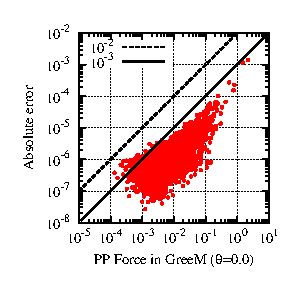
\includegraphics[width=10cm,bb=0 0 170 170]{fig/comparison_pp.eps}
  \end{center}
  \caption{GreeMのPP forceの絶対値(横軸)と, GreeMとFDPSのPP forceの絶対
    誤差(縦軸). ツリーの精度は$\theta=0.0$.}
  \label{fig:comparison_pp}
\end{figure}

\begin{figure}
  \begin{center}
    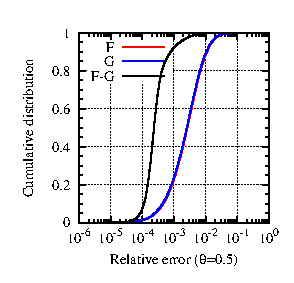
\includegraphics[width=10cm,bb=0 0 170 170]{fig/comparison_pt05.eps}
  \end{center}
  \caption{(赤)FDPSのPP forceの相対誤差($\theta=0.0$と$0.5$を比較).
    (青)GreeMのPP forceの相対誤差($\theta=0.0$と$0.5$を比較). (黒)FDPS
    とGreeMのPP forceの相対誤差(どちらも$\theta=0.5$).}
  \label{fig:comparison_pt05}
\end{figure}

\begin{figure}
  \begin{center}
    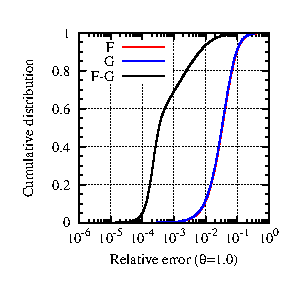
\includegraphics[width=10cm,bb=0 0 170 170]{fig/comparison_pt10.eps}
  \end{center}
  \caption{(赤)FDPSのPP forceの相対誤差($\theta=0.0$と$1.0$を比較).
    (青)GreeMのPP forceの相対誤差($\theta=0.0$と$1.0$を比較). (黒)FDPS
    とGreeMのPP forceの相対誤差(どちらも$\theta=1.0$).}
  \label{fig:comparison_pt10}
\end{figure}

